
\chapter{Computational Implementation}\label{implementation}

A computational method for inverter impedance calculation is introduced and implemented in this study and presented in this chapter. The computational approach is chosen to handle the sizeable parametric matrix calculations and prevent human error during model calculations. First, the computational procedure is explained, and later, the resultant models are presented for each inverter of \ref{Inverters}.

\section{Computational Procedure}

In \ref{smallsignal} all block equations are finally converted into matrix form with $2 \times 2$ parameters and $1 \times 2$ variables. With this kind of mapping, without loss of generality, all the blocks can be put into a set of algebraic equations of scalar parameters and scalar variables and can be solved via scalar equation solvers. The results of this derivation are presented in \ref{formula}. Because these results can be saved once and used later rather than solving the equation each time, this approach is computationally efficient. After saving the results, the variables will be eliminated, and $2 \times 2$ parameters are plugged to result into a final admittance/impedance $2 \times 2$ parameter. After this calculation, the results of each component, $dd$, $dq$, $qd$, and $qq$, for each inverter are saved separately, preferably as a character data class in the computer. Finally, the latter formulas can be used for each instance of parameters to derive the numerical transfer functions.

\section{Small Signal Impedance Results}\label{formula}

The algebraic solution of matrix equation for each inverter is presented here:

For the \gls{GFM} inverters the nominators and denominators are presented separately due to their complexity.

\subsubsection{Grid Following Inverter: Conventional Model}
\begin{center}
\begin{equation}\label{4}
Z_{GFL}=
\frac
{
\begin{split}
Z_L_1 - Z_L_2 - Deld*Kdc - Delv*L1w\\ + Delv*PIC + Delv*FV*Z_L_2 + Deld*Ydc*Z_L_2\\ + Z_c*Z_L_1*Z_L_2 + Delv*PIC*PIS*V - Delv*L1w*Z_c*Z_L_2\\ + Delv*PIC*Z_c*Z_L_2 - Delv*I*PIC*PIS*Z_L_2
\end{split}}
{\begin{split}Z_c*Z_L_1 + Delv*FV + Deld*Ydc\\ - Delv*L1w*Z_c + Delv*PIC*Z_c - Delv*I*PIC*PIS - 1\end{split}}
\end{equation}
\end{center}


\pagebreak
\subsubsection{Grid Following Inverter: Exact Model}
\begin{center}
\begin{equation}\label{4}
Z_{GFL-Exact}=
\frac
{
\begin{split}
Z_L_1 - Z_L_2 - Delv*L1w + Delv*PIC\\ + Delv*FV*Z_L_2 - PLL*Tv*Z_L_1 +\\ PLL*Tv*Z_L_2 + Z_c*Z_L_1*Z_L_2 + Delv*L1w*PLL*Tv -\\ Delv*PIC*PLL*Tv - Delv*L1w*Z_c*Z_L_2 +\\ Delv*PIC*Z_c*Z_L_2 - PLL*Tv*Z_c*Z_L_1*Z_L_2 +\\ Delv*Droop*PIC*PIS*Z_L_2 +Delv*PFilter*PIC*PIS*V +\\ Delv*L1w*PLL*Ti*Z_L_2 -Delv*PIC*PLL*Ti*Z_L_2\\+ Delv*PLL*Td*Tmain*Z_L_2 - Delv*I*PFilter*PIC*PIS*Z_L_2\\+ Delv*L1w*PLL*Tv*Z_c*Z_L_2\\ - Delv*PIC*PLL*Tv*Z_c*Z_L_2\\ - Delv*PFilter*PIC*PIS*PLL*Tv*V\\ - Delv*PFilter*PIC*PIS*PLL*Tio*V*Z_L_2
\end{split}}
{\begin{split}PLL*Tv + Z_c*Z_L_1 + Delv*FV\\ - Delv*L1w*Z_c + Delv*PIC*Z_c\\+ Delv*Droop*PIC*PIS\\ + Delv*L1w*PLL*Ti - Delv*PIC*PLL*Ti +\\ Delv*PLL*Td*Tmain\\ - PLL*Tv*Z_c*Z_L_1 -\\Delv*I*PFilter*PIC*PIS + Delv*L1w*PLL*Tv*Z_c -\\ Delv*PIC*PLL*Tv*Z_c\\ - Delv*PFilter*PIC*PIS*PLL*Tio*V - 1\end{split}}
\end{equation}
\end{center}


\pagebreak
\subsubsection{Grid Forming Inverter: Droop Control}
\begin{equation}\label{DroopNum}
$Z_{GFM-droop}(Nominator)=Z_L_1 - Z_L_2 - Delv*L1w + Delv*PIC - Cw*Delv*PIC - Delv*FII*PIC + Delv*FV*Z_L_2 + Z_c*Z_L_1*Z_L_2 - Delv*PIC*PIV*Z_L_2 - Delv*L1w*Z_c*Z_L_2 + Delv*PIC*Z_c*Z_L_2 - Cw*Delv*PIC*Z_c*Z_L_2 - DroopGFM*I*PFilter*Tv*Z_L_1 + DroopGFM*I*PFilter*Tv*Z_L_2 - Delv*FII*PIC*Z_c*Z_L_2 - DroopGFM*PFilter*Tio*V*Z_L_1 + DroopGFM*PFilter*Tio*V*Z_L_2 + Delv*DroopGFM*I*L1w*PFilter*Tv - Delv*DroopGFM*I*PFilter*PIC*Tv - Delv*DroopGFM*FV*PFilter*Tv*V - Delv*DroopGFM*L1w*PFilter*Ti*V + Delv*DroopGFM*L1w*PFilter*Tio*V + Delv*DroopGFM*PFilter*PIC*Ti*V - Delv*DroopGFM*PFilter*PIC*Tio*V - Delv*DroopGFM*PFilter*Td*Tmain*V + Cw*Delv*DroopGFM*I*PFilter*PIC*Tv + Delv*DroopGFM*FII*I*PFilter*PIC*Tv - Cw*Delv*DroopGFM*PFilter*PIC*Ti*V + Cw*Delv*DroopGFM*PFilter*PIC*Tio*V - Delv*DroopGFM*FII*PFilter*PIC*Ti*V + Delv*DroopGFM*FII*PFilter*PIC*Tio*V + Delv*DroopGFM*I*L1w*PFilter*Ti*Z_L_2 - Delv*DroopGFM*I*PFilter*PIC*Ti*Z_L_2 + Delv*DroopGFM*PFilter*PIC*PIV*Tv*V - Delv*DroopGFM*FV*PFilter*Tio*V*Z_L_2 + Delv*DroopGFM*I*PFilter*Td*Tmain*Z_L_2 - DroopGFM*I*PFilter*Tv*Z_c*Z_L_1*Z_L_2 - DroopGFM*PFilter*Tio*V*Z_c*Z_L_1*Z_L_2 + Cw*Delv*DroopGFM*I*PFilter*PIC*Ti*Z_L_2 + Delv*DroopGFM*FII*I*PFilter*PIC*Ti*Z_L_2 + Delv*DroopGFM*I*L1w*PFilter*Tv*Z_c*Z_L_2 - Delv*DroopGFM*I*PFilter*PIC*Tv*Z_c*Z_L_2 + Delv*DroopGFM*PFilter*PIC*PIV*Tio*V*Z_L_2 + Delv*DroopGFM*L1w*PFilter*Tio*V*Z_c*Z_L_2 - Delv*DroopGFM*PFilter*PIC*Tio*V*Z_c*Z_L_2 + Cw*Delv*DroopGFM*I*PFilter*PIC*Tv*Z_c*Z_L_2 + Delv*DroopGFM*FII*I*PFilter*PIC*Tv*Z_c*Z_L_2 + Cw*Delv*DroopGFM*PFilter*PIC*Tio*V*Z_c*Z_L_2 + Delv*DroopGFM*FII*PFilter*PIC*Tio*V*Z_c*Z_L_2$    
\end{equation}

    

\begin{equation}\label{DroopDen}
$Z_{GFM-droop}(Denominator)=Z_c*Z_L_1 + Delv*FV - Delv*PIC*PIV - Delv*L1w*Z_c + Delv*PIC*Z_c - Cw*Delv*PIC*Z_c + DroopGFM*I*PFilter*Tv - Delv*FII*PIC*Z_c + DroopGFM*PFilter*Tio*V + Delv*DroopGFM*I*L1w*PFilter*Ti - Delv*DroopGFM*I*PFilter*PIC*Ti - Delv*DroopGFM*FV*PFilter*Tio*V + Delv*DroopGFM*I*PFilter*Td*Tmain - DroopGFM*I*PFilter*Tv*Z_c*Z_L_1 - DroopGFM*PFilter*Tio*V*Z_c*Z_L_1 + Cw*Delv*DroopGFM*I*PFilter*PIC*Ti + Delv*DroopGFM*FII*I*PFilter*PIC*Ti + Delv*DroopGFM*I*L1w*PFilter*Tv*Z_c - Delv*DroopGFM*I*PFilter*PIC*Tv*Z_c + Delv*DroopGFM*PFilter*PIC*PIV*Tio*V + Delv*DroopGFM*L1w*PFilter*Tio*V*Z_c - Delv*DroopGFM*PFilter*PIC*Tio*V*Z_c + Cw*Delv*DroopGFM*I*PFilter*PIC*Tv*Z_c + Delv*DroopGFM*FII*I*PFilter*PIC*Tv*Z_c + Cw*Delv*DroopGFM*PFilter*PIC*Tio*V*Z_c + Delv*DroopGFM*FII*PFilter*PIC*Tio*V*Z_c - 1$   
\end{equation}
\pagebreak
\subsubsection{Grid Forming Inverter: Power Synchronization Loop}

\begin{equation}\label{PSCNum}
    $Z_{GFM-PSC}(Nominator)=Z_L_1 - Z_L_2 - Delv*L1w + Delv*PIC - Cw*Delv*PIC - Delv*FII*PIC + Delv*FV*Z_L_2 + Z_c*Z_L_1*Z_L_2 - Delv*PIC*PIV*Z_L_2 - Delv*L1w*Z_c*Z_L_2 + Delv*PIC*Z_c*Z_L_2 - PFilter*PSC*Tio*V*Z_L_1 + PFilter*PSC*Tio*V*Z_L_2 - Cw*Delv*PIC*Z_c*Z_L_2 - Delv*FII*PIC*Z_c*Z_L_2 - I*PFilter*PSC*Tv*Z_L_1 + I*PFilter*PSC*Tv*Z_L_2 + Delv*I*L1w*PFilter*PSC*Tv - Delv*I*PFilter*PIC*PSC*Tv - Delv*FV*PFilter*PSC*Tv*V - Delv*L1w*PFilter*PSC*Ti*V + Delv*L1w*PFilter*PSC*Tio*V + Delv*PFilter*PIC*PSC*Ti*V - Delv*PFilter*PIC*PSC*Tio*V - Delv*PFilter*PSC*Td*Tmain*V + Cw*Delv*I*PFilter*PIC*PSC*Tv + Delv*FII*I*PFilter*PIC*PSC*Tv - Cw*Delv*PFilter*PIC*PSC*Ti*V + Cw*Delv*PFilter*PIC*PSC*Tio*V - Delv*FII*PFilter*PIC*PSC*Ti*V + Delv*FII*PFilter*PIC*PSC*Tio*V + Delv*I*L1w*PFilter*PSC*Ti*Z_L_2 - Delv*I*PFilter*PIC*PSC*Ti*Z_L_2 + Delv*PFilter*PIC*PIV*PSC*Tv*V - Delv*FV*PFilter*PSC*Tio*V*Z_L_2 + Delv*I*PFilter*PSC*Td*Tmain*Z_L_2 - I*PFilter*PSC*Tv*Z_c*Z_L_1*Z_L_2 - PFilter*PSC*Tio*V*Z_c*Z_L_1*Z_L_2 + Cw*Delv*I*PFilter*PIC*PSC*Ti*Z_L_2 + Delv*FII*I*PFilter*PIC*PSC*Ti*Z_L_2 + Delv*I*L1w*PFilter*PSC*Tv*Z_c*Z_L_2 - Delv*I*PFilter*PIC*PSC*Tv*Z_c*Z_L_2 + Delv*PFilter*PIC*PIV*PSC*Tio*V*Z_L_2 + Delv*L1w*PFilter*PSC*Tio*V*Z_c*Z_L_2 - Delv*PFilter*PIC*PSC*Tio*V*Z_c*Z_L_2 + Cw*Delv*I*PFilter*PIC*PSC*Tv*Z_c*Z_L_2 + Delv*FII*I*PFilter*PIC*PSC*Tv*Z_c*Z_L_2 + Cw*Delv*PFilter*PIC*PSC*Tio*V*Z_c*Z_L_2 + Delv*FII*PFilter*PIC*PSC*Tio*V*Z_c*Z_L_2$
\end{equation}


\begin{equation}\label{PSCDen}
   $Z_{GFM-PSC}(Denominator)=Z_c*Z_L_1 + Delv*FV - Delv*PIC*PIV - Delv*L1w*Z_c + Delv*PIC*Z_c - Cw*Delv*PIC*Z_c - Delv*FII*PIC*Z_c + I*PFilter*PSC*Tv + PFilter*PSC*Tio*V + Delv*I*L1w*PFilter*PSC*Ti - Delv*I*PFilter*PIC*PSC*Ti - Delv*FV*PFilter*PSC*Tio*V + Delv*I*PFilter*PSC*Td*Tmain - I*PFilter*PSC*Tv*Z_c*Z_L_1 - PFilter*PSC*Tio*V*Z_c*Z_L_1 + Cw*Delv*I*PFilter*PIC*PSC*Ti + Delv*FII*I*PFilter*PIC*PSC*Ti + Delv*I*L1w*PFilter*PSC*Tv*Z_c - Delv*I*PFilter*PIC*PSC*Tv*Z_c + Delv*PFilter*PIC*PIV*PSC*Tio*V + Delv*L1w*PFilter*PSC*Tio*V*Z_c - Delv*PFilter*PIC*PSC*Tio*V*Z_c + Cw*Delv*I*PFilter*PIC*PSC*Tv*Z_c + Delv*FII*I*PFilter*PIC*PSC*Tv*Z_c + Cw*Delv*PFilter*PIC*PSC*Tio*V*Z_c + Delv*FII*PFilter*PIC*PSC*Tio*V*Z_c - 1$ 
\end{equation}
\pagebreak
\subsubsection{Grid Forming Inverter: Synchronvector}

\begin{equation}\label{SYNNum}
$Z_{GFM-SYN}(Nominator)=Z_L_1 - Z_L_2 - Delv*L1w + Delv*PIC - Cw*Delv*PIC - Delv*FII*PIC + Delv*FV*Z_L_2 + Z_c*Z_L_1*Z_L_2 - Delv*PIC*PIV*Z_L_2 - Delv*L1w*Z_c*Z_L_2 + Delv*PIC*Z_c*Z_L_2 - PFilter*SYN*Tio*V*Z_L_1 + PFilter*SYN*Tio*V*Z_L_2 - Cw*Delv*PIC*Z_c*Z_L_2 - Delv*FII*PIC*Z_c*Z_L_2 - I*PFilter*SYN*Tv*Z_L_1 + I*PFilter*SYN*Tv*Z_L_2 + Delv*I*L1w*PFilter*SYN*Tv - Delv*I*PFilter*PIC*SYN*Tv - Delv*FV*PFilter*SYN*Tv*V - Delv*L1w*PFilter*SYN*Ti*V + Delv*L1w*PFilter*SYN*Tio*V + Delv*PFilter*PIC*SYN*Ti*V - Delv*PFilter*PIC*SYN*Tio*V - Delv*PFilter*SYN*Td*Tmain*V + Cw*Delv*I*PFilter*PIC*SYN*Tv + Delv*FII*I*PFilter*PIC*SYN*Tv - Cw*Delv*PFilter*PIC*SYN*Ti*V + Cw*Delv*PFilter*PIC*SYN*Tio*V - Delv*FII*PFilter*PIC*SYN*Ti*V + Delv*FII*PFilter*PIC*SYN*Tio*V + Delv*I*L1w*PFilter*SYN*Ti*Z_L_2 - Delv*I*PFilter*PIC*SYN*Ti*Z_L_2 + Delv*PFilter*PIC*PIV*SYN*Tv*V - Delv*FV*PFilter*SYN*Tio*V*Z_L_2 + Delv*I*PFilter*SYN*Td*Tmain*Z_L_2 - I*PFilter*SYN*Tv*Z_c*Z_L_1*Z_L_2 - PFilter*SYN*Tio*V*Z_c*Z_L_1*Z_L_2 + Cw*Delv*I*PFilter*PIC*SYN*Ti*Z_L_2 + Delv*FII*I*PFilter*PIC*SYN*Ti*Z_L_2 + Delv*I*L1w*PFilter*SYN*Tv*Z_c*Z_L_2 - Delv*I*PFilter*PIC*SYN*Tv*Z_c*Z_L_2 + Delv*PFilter*PIC*PIV*SYN*Tio*V*Z_L_2 + Delv*L1w*PFilter*SYN*Tio*V*Z_c*Z_L_2 - Delv*PFilter*PIC*SYN*Tio*V*Z_c*Z_L_2 + Cw*Delv*I*PFilter*PIC*SYN*Tv*Z_c*Z_L_2 + Delv*FII*I*PFilter*PIC*SYN*Tv*Z_c*Z_L_2 + Cw*Delv*PFilter*PIC*SYN*Tio*V*Z_c*Z_L_2 + Delv*FII*PFilter*PIC*SYN*Tio*V*Z_c*Z_L_2$  
\end{equation}

\begin{equation}\label{SYNDen}
   $Z_{GFM-SYN}(Denominator)=Z_c*Z_L_1 + Delv*FV - Delv*PIC*PIV - Delv*L1w*Z_c + Delv*PIC*Z_c - Cw*Delv*PIC*Z_c - Delv*FII*PIC*Z_c + I*PFilter*SYN*Tv + PFilter*SYN*Tio*V + Delv*I*L1w*PFilter*SYN*Ti - Delv*I*PFilter*PIC*SYN*Ti - Delv*FV*PFilter*SYN*Tio*V + Delv*I*PFilter*SYN*Td*Tmain - I*PFilter*SYN*Tv*Z_c*Z_L_1 - PFilter*SYN*Tio*V*Z_c*Z_L_1 + Cw*Delv*I*PFilter*PIC*SYN*Ti + Delv*FII*I*PFilter*PIC*SYN*Ti + Delv*I*L1w*PFilter*SYN*Tv*Z_c - Delv*I*PFilter*PIC*SYN*Tv*Z_c + Delv*PFilter*PIC*PIV*SYN*Tio*V + Delv*L1w*PFilter*SYN*Tio*V*Z_c - Delv*PFilter*PIC*SYN*Tio*V*Z_c + Cw*Delv*I*PFilter*PIC*SYN*Tv*Z_c + Delv*FII*I*PFilter*PIC*SYN*Tv*Z_c + Cw*Delv*PFilter*PIC*SYN*Tio*V*Z_c + Delv*FII*PFilter*PIC*SYN*Tio*V*Z_c - 1$ 
\end{equation}
\pagebreak
\subsubsection{Grid Forming Inverter: Virtual Inertia}

\begin{equation}\label{VILNum}
$Z_{GFM-VIL}(Nominator)=Z_L_1 - Z_L_2 - Delv*L1w + Delv*PIC - Cw*Delv*PIC - Delv*FII*PIC + Delv*FV*Z_L_2 + Z_c*Z_L_1*Z_L_2 - Delv*PIC*PIV*Z_L_2 - Delv*L1w*Z_c*Z_L_2 + Delv*PIC*Z_c*Z_L_2 - PFilter*Tio*V*VIL*Z_L_1 + PFilter*Tio*V*VIL*Z_L_2 - Cw*Delv*PIC*Z_c*Z_L_2 - Delv*FII*PIC*Z_c*Z_L_2 - I*PFilter*Tv*VIL*Z_L_1 + I*PFilter*Tv*VIL*Z_L_2 + Delv*I*L1w*PFilter*Tv*VIL - Delv*I*PFilter*PIC*Tv*VIL - Delv*FV*PFilter*Tv*V*VIL - Delv*L1w*PFilter*Ti*V*VIL + Delv*L1w*PFilter*Tio*V*VIL + Delv*PFilter*PIC*Ti*V*VIL - Delv*PFilter*PIC*Tio*V*VIL - Delv*PFilter*Td*Tmain*V*VIL + Cw*Delv*I*PFilter*PIC*Tv*VIL + Delv*FII*I*PFilter*PIC*Tv*VIL - Cw*Delv*PFilter*PIC*Ti*V*VIL + Cw*Delv*PFilter*PIC*Tio*V*VIL - Delv*FII*PFilter*PIC*Ti*V*VIL + Delv*FII*PFilter*PIC*Tio*V*VIL + Delv*I*L1w*PFilter*Ti*VIL*Z_L_2 - Delv*I*PFilter*PIC*Ti*VIL*Z_L_2 + Delv*PFilter*PIC*PIV*Tv*V*VIL - Delv*FV*PFilter*Tio*V*VIL*Z_L_2 + Delv*I*PFilter*Td*Tmain*VIL*Z_L_2 - I*PFilter*Tv*VIL*Z_c*Z_L_1*Z_L_2 - PFilter*Tio*V*VIL*Z_c*Z_L_1*Z_L_2 + Cw*Delv*I*PFilter*PIC*Ti*VIL*Z_L_2 + Delv*FII*I*PFilter*PIC*Ti*VIL*Z_L_2 + Delv*I*L1w*PFilter*Tv*VIL*Z_c*Z_L_2 - Delv*I*PFilter*PIC*Tv*VIL*Z_c*Z_L_2 + Delv*PFilter*PIC*PIV*Tio*V*VIL*Z_L_2 + Delv*L1w*PFilter*Tio*V*VIL*Z_c*Z_L_2 - Delv*PFilter*PIC*Tio*V*VIL*Z_c*Z_L_2 + Cw*Delv*I*PFilter*PIC*Tv*VIL*Z_c*Z_L_2 + Delv*FII*I*PFilter*PIC*Tv*VIL*Z_c*Z_L_2 + Cw*Delv*PFilter*PIC*Tio*V*VIL*Z_c*Z_L_2 + Delv*FII*PFilter*PIC*Tio*V*VIL*Z_c*Z_L_2$  
\end{equation}

\pagebreak

\begin{equation}\label{VILDen}
    $Z_{GFM-VIL}(Denominator)=Z_c*Z_L_1 + Delv*FV - Delv*PIC*PIV - Delv*L1w*Z_c + Delv*PIC*Z_c - Cw*Delv*PIC*Z_c - Delv*FII*PIC*Z_c + I*PFilter*Tv*VIL + PFilter*Tio*V*VIL + Delv*I*L1w*PFilter*Ti*VIL - Delv*I*PFilter*PIC*Ti*VIL - Delv*FV*PFilter*Tio*V*VIL + Delv*I*PFilter*Td*Tmain*VIL - I*PFilter*Tv*VIL*Z_c*Z_L_1 - PFilter*Tio*V*VIL*Z_c*Z_L_1 + Cw*Delv*I*PFilter*PIC*Ti*VIL + Delv*FII*I*PFilter*PIC*Ti*VIL + Delv*I*L1w*PFilter*Tv*VIL*Z_c - Delv*I*PFilter*PIC*Tv*VIL*Z_c + Delv*PFilter*PIC*PIV*Tio*V*VIL + Delv*L1w*PFilter*Tio*V*VIL*Z_c - Delv*PFilter*PIC*Tio*V*VIL*Z_c + Cw*Delv*I*PFilter*PIC*Tv*VIL*Z_c + Delv*FII*I*PFilter*PIC*Tv*VIL*Z_c + Cw*Delv*PFilter*PIC*Tio*V*VIL*Z_c + Delv*FII*PFilter*PIC*Tio*V*VIL*Z_c - 1$
\end{equation}


\section{Matrix Substitution}

In the next step, each term of the above equations is replaced with its corresponding complex matrix. A list of All Terms with their Complex form is presented in \cref{tbl1,tbl2}.

\begin{table}[ht]
\centering
\caption[Matrix Substitution Parameters 1]{Matrix Arrays of Parameters}
\label{tbl1}
\resizebox{.8\textwidth}{!}{%
\begin{tabular}{lllll}
\hline
Parameter & dd & dq & qd & qq \\ \hline
Vo & V_{do} & V_{qo} & V_{qo} & -V_{do} \\
Io & I_{do} & I_{qo} & -I_{qo} & I_{do} \\
Z_L_1 & sL_1 & -\omega L_1 & \omega L_1 & sL_1 \\
L1w & 0 & -\omega L_1 & \omega L_1 & 0 \\
Z_L_2 & sL_2 & -\omega L_2 & \omega L_2 & sL_2 \\
L2w & 0 & -\omega L_1 & \omega L_1 & 0 \\
Z_c & sC & -\omega C & \omega C & sC \\
Cw & 0 & -\omega C & \omega C & 0 \\
PIC & KP_c+KI_c/s & 0 & 0 & KP_c+KI_c/s \\
Fv & K_{vf}/{(1+T_{vf}s)} & 0 & 0 & K_{vf}/{(1+T_{vf}s)} \\
FII & K_{vii}/{(1+T_{vii}s)} & 0 & 0 & K_{vii}/{(1+T_{vii}s)} \\
PIS & KP_p+KI_p/s & 0 & 0 & KP_q+KI_q/s \\
PIV & KP_pV+KI_pV/s & 0 & 0 & KP_qV+KI_qV/s \\
PFilter & \omega_c/{s+\omega_c} & 0 & 0 & \omega_c/{s+\omega_c} \\
PLL & 0 & 0 & 0 & KP_{pll}+KI_{pll}/s \\
Droop & 0 & KP_{pll}+KI_{pll}/s & V_d/{n\sqrt{V_d^2+V_q^2}} & V_q/{n\sqrt{V_d^2+V_q^2}} \\

%Y_{DC} & 0 & 0 & 0 & 0 \\
\hline
\end{tabular}
}
\end{table}

\begin{table}[ht]
\centering
\caption[Matrix Substitution Parameters 2]{Matrix Arrays of Parameters}

\label{tbl2}
\resizebox{.8\textwidth}{!}{%
\begin{tabular}{lllll}
\hline
Parameter  & dd & dq & qd & qq \\ \hline
DroopGFL &$ D_f/s $& $D_f/s$ & 0 & 0 \\
VIL & $1/(Js^2+D_{vil}s)$ & $1/(Js^2+D_{vil}s)$ & 0 & 0 \\
SYN &  $\frac{1}{sJ\omega_n(s+\frac{D_p}{J(1+D_pPI_ps)})}$  & $\frac{1}{sJ\omega_n(s+\frac{D_p}{J(1+D_pPI_ps)})}$  & 0 & 0\\
PSC & $K_pSC/s$ & $K_pSC/s$ & 0 & 0 \\
K_{DC} & $I_d/{C_{DC}V_{DC}}$ & $I_q/{C_{DC}V_{DC}}$ & 0 & 0 \\
Y_{DC} & $V_d/{C_{DC}V_{DC}}$ & $V_q/{C_{DC}V_{DC}}$ & 0 & 0 \\
DelD & $D(\frac{1-0.5T_{del}s}{1+0.5T_{del}s})$ & 0 & 0 & $D(\frac{1-0.5T_{del}s}{1+0.5T_{del}s})$ \\
Delv & $Vdc(\frac{1-0.5T_{del}s}{1+0.5T_{del}s})$ & 0 & 0 & $Vdc(\frac{1-0.5T_{del}s}{1+0.5T_{del}s})$ \\
TETA & $cos(\theta)$ & $sin(\theta)$ & $-sin(\theta)$ & $cos(\theta)$ \\
T_v & 0 & $-sin(\theta)V_d+cos(\theta)V_q$  & 0 & $-cos(\theta)I_d-sin(\theta)I_q$ \\
T_{io} & 0 & $-sin(\theta)Io_d+cos(\theta)Io_q$  & 0 & $-cos(\theta)Io_d-sin(\theta)Io_q$ \\
T_i & 0 & $-sin(\theta)I_d+cos(\theta)I_q$  & 0 & $-cos(\theta)I_d-sin(\theta)I_q$ \\
T_d & 0 & $cos(\theta)D_d+sin(\theta)D_q$ & 0 & $-sin(\theta) D_d+cos(\theta)D_q$ \\
\hline
\end{tabular}
}
\end{table}

\section{Parameters Substitution and Tuning}\label{parameters}


\begin{figure}[ht]
    \centering
	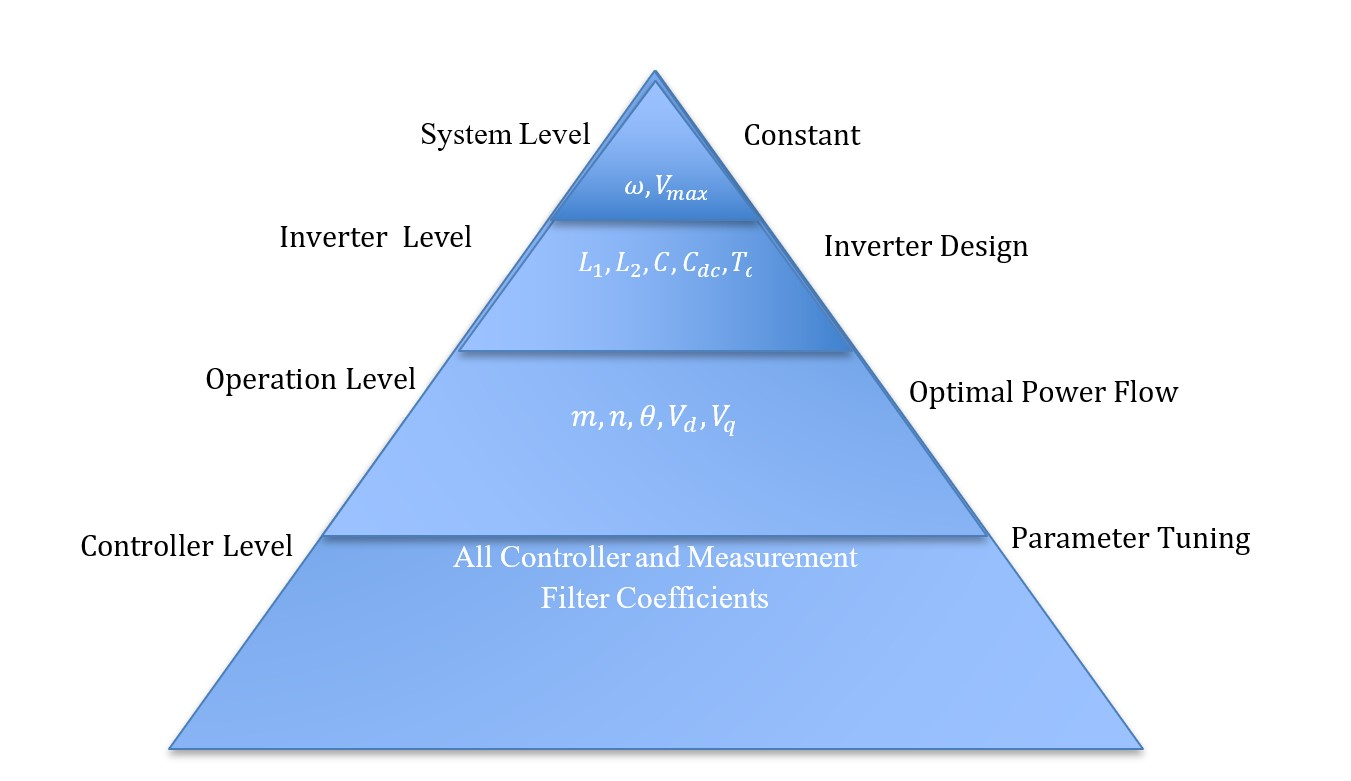
\includegraphics[width=0.85\textwidth]{figures/Hierarchy.jpg}
	\caption[Hierarchy of Small Signal Derivation]{Hierarchy of Small Signal Derivation}
	\label{fig:hr}
\end{figure}


After matrix substitution, Four parametric transfer functions will be generated for each of the inverters of \ref{Inverters}. Some of these parameters, such as system frequency $\omega$ are determined by the system. Whereas, semiconductor, LCL, and DC elements ($L_1$, $L_2$, $C$, and $C_{DC}$ and $T_{del}$), are determined via inverter hardware design process. In addition, voltage magnitude and angle reference, which are not dependent on each other ($tan\theta=V_q/V_d$) and also \gls{GFM} droop control coefficients are determined via grid operation. Finally, the rest of the coefficients are implemented locally on a control board. In this design hierarchy, the goal is to achieve the best performance with the given parameters of an upper-level study. However, upper-level adjustments are required if the goal cannot be achieved. Although there are systematic methods such as \cite{ParamTune} to search for the best parameters, they are limited to a particular type of inverter and also are designed for a more limited inverter model. In the \ref{results} an approach has been made to tune these parameters. \ref{fig:hr} summarizes the parameters of small-signal modeling and their corresponding study.